%% TrashScribe -- manuscript for Neural Computing and Applications,
%% Topical Collection "Emerging Trends in Smart Waste Monitoring and Environmental Surveillance".
%% ANONYMISED for double-blind review: author data live in title_page.tex only.
%% Red [bracketed] text marks what must be filled from runs (scripts/make_tables.py, list_runs.py).
\documentclass[pdflatex,sn-basic,Numbered]{sn-jnl}% Basic SN style, numbered citations [1] as required by NCAA

\usepackage{graphicx}%
\usepackage{multirow}%
\usepackage{amsmath,amssymb,amsfonts}%
\usepackage{xcolor}%
\usepackage{textcomp}%
\usepackage{booktabs}%
\usepackage{tikz}%
\usetikzlibrary{arrows.meta,positioning,fit,calc}%

\newcommand{\tbd}[1]{\textcolor{red}{[#1]}}
\newcommand{\trashscribe}{TrashScribe}
% \input is robust (non-expandable) since LaTeX 2020 and breaks \midrule inside tabulars
\makeatletter\newcommand{\tabinput}[1]{\@@input #1 }\makeatother

\raggedbottom

\begin{document}

\title[Attribute-grounded, environment-agnostic waste segmentation on the edge]{TrashScribe: Describing Waste Instead of Naming It --- Attribute-Grounded, Environment-Agnostic Waste Segmentation for Offline Monitoring on the Edge}

%% double-blind: no author information in the manuscript
\author{\fnm{Anonymous} \sur{Author(s)}}
\affil{\orgname{Anonymous Institution(s)}}

\abstract{Smart waste monitoring needs vision systems that work wherever waste lies---streets, beaches, rivers, recycling plants---often on devices without connectivity. Waste segmentation models are usually trained and tested on one dataset at a time, with a closed taxonomy, and tend to learn the environment as much as the waste. We present \trashscribe{}, a waste segmentation and description system built on three principles. First, a single prompt-free decoder on a frozen SAM2-Hiera-Tiny encoder, adapted through zero-initialised adapters, answers the only question every dataset annotates: which pixels are waste. Second, instead of predicting classes, a dense descriptor field grounds each object in a controlled vocabulary of visual properties---material, rigidity, optical behaviour, shape, surface---scored in a frozen text space with no per-descriptor or per-class parameter; classes, municipal sorting streams and new waste types are written in an atlas and read at inference. Third, object evidence is pooled inside the mask while context is pooled in a surrounding ring and never used for naming, and a cross-dataset object transplant with an environment adversary removes the background shortcut. We evaluate on five public datasets (TACO, ZeroWaste-f, UAVVaste, MJU-Waste, BePLi v2) under a leave-one-dataset-out protocol, with seven TACO classes held out of every training stage. \tbd{One sentence with the main LODO IoU gain over the strongest baseline, descriptor mAP over the prevalence floor, and held-out retrieval lift.} The whole network runs as one TensorRT engine on a Jetson Orin Nano 8\,GB at \tbd{XX}\,ms per frame, fully offline.}

\keywords{Smart waste monitoring, Domain generalisation, Open-vocabulary segmentation, Attribute-based zero-shot learning, Edge AI, Segment Anything}

\maketitle

%% ============================================================================
\section{Introduction}\label{sec:intro}

Waste that escapes collection---litter on streets and beaches, illegal dumps at the edge of towns, objects mis-sorted on a recycling line---is cheap to photograph and expensive to count. Cameras on collection vehicles, drones, fixed poles and sorting plants already produce the images; what limits automatic monitoring is a vision model that keeps working when the camera, the place and the waste change, and that runs where the images are taken, often without a network connection.

Current waste segmentation methods do not meet these conditions for three reasons. First, they are trained and evaluated within a single dataset~\cite{proenca2020taco,bashkirova2022zerowaste,wang2020mjuwaste,aboubaker2023dontwaste,javaid2026cluttered}. Each public dataset covers one environment---a conveyor belt~\cite{bashkirova2022zerowaste}, a beach~\cite{bepli2023}, an aerial view~\cite{kraft2021uavvaste}, a street~\cite{paulo2026streetview}---so in-domain accuracy says little about a deployment elsewhere, and the one challenge that measured the shift stayed inside the same industrial domain~\cite{bashkirova2023visda}. Second, they predict a closed set of classes. Taxonomies disagree across datasets (60 fine classes in TACO, four in ZeroWaste, a single ``waste'' class in UAVVaste and MJU-Waste) and across municipalities, whose sorting rules group materials differently; adding a waste type costs a new annotated image set and a retraining. Open-vocabulary detectors relax the vocabulary over object \emph{names}, but on waste they need carefully engineered prompts and still trail supervised models~\cite{abid2025robustwaste}. Third, in every dataset the object and its surroundings are correlated---cardboard on the conveyor, fragments on the sand, cans on the pavement---so a model can ``recognise'' a material from the background and fail as soon as the background changes.

We address the three problems with one design principle, borrowed from how an operator reads a scene: \emph{find} waste, \emph{describe} it, and only then \emph{name} it, by reading a description written for humans. Finding is the only question every dataset annotates, so it is trained on all of them together. Describing uses a vocabulary of visual properties (material, rigidity, optical behaviour, shape, surface, colour, state, size) that is shared by every taxonomy; a class is a composition of such properties, so a class never seen in training can still be described with words that were. Naming is a lookup in a text file, the \emph{atlas}, that contributes no parameter to the model. This separation follows recent work on descriptor-based retrieval in diagnostic microscopy~\cite{anon_mirf}, which we transfer from object crops to dense segmentation and extend with explicit control of the environment.

The resulting system, \trashscribe{}\footnote{A scribe for trash: the system writes a description of every piece of waste and reads names from text, rather than assigning it a class.}, makes the following contributions:
\begin{enumerate}
\item A parameter-efficient segmentation architecture for heterogeneous waste data: a frozen SAM2-Hiera-Tiny encoder~\cite{ravi2025sam2,ryali2023hiera} adapted with zero-initialised adapters, a prompt-free waste decoder shared by every dataset, a contour head that splits touching objects without per-object decoder calls, and an optional geometric gate driven by depth that starts as the identity (Sect.~\ref{sec:where}).
\item A dense descriptor field projected into a frozen text space and scored with no per-descriptor or per-class parameter, so that the vocabulary, the classes and the sorting streams can be extended at inference by editing text (Sects.~\ref{sec:what}--\ref{sec:naming}).
\item An environment-agnostic training scheme: intrinsic evidence pooled inside each mask and contextual evidence in a ring around it, never used for naming; cross-dataset object transplant; an environment adversary with gradient reversal; feature-statistics mixing; and an environment-leakage probe that measures what remains (Sect.~\ref{sec:debias}).
\item A leave-one-dataset-out benchmark over five public waste datasets with seven classes held out of every training stage, evaluated as segmentation, description, generalised zero-shot naming and retrieval (Sect.~\ref{sec:setup}), and an offline deployment on a Jetson Orin Nano 8\,GB (Sect.~\ref{sec:edge}).
\end{enumerate}

Source code, configuration files for every experiment and the atlases are available at \tbd{anonymised repository URL}.

%% ============================================================================
\section{Related work}\label{sec:related}

\subsection{Waste datasets and segmentation}
TACO~\cite{proenca2020taco} collects 1{,}500 photographs of litter in the wild with 4{,}784 instance masks over 60 classes and per-image scene labels. ZeroWaste~\cite{bashkirova2022zerowaste} targets deformable, cluttered objects on a recycling conveyor with four classes and labelled and unlabelled splits; its domain adaptation challenge~\cite{bashkirova2023visda} showed that augmentation and ensembling help across two plants. MJU-Waste~\cite{wang2020mjuwaste} adds depth in indoor scenes, UAVVaste~\cite{kraft2021uavvaste} aerial litter, BePLi~\cite{bepli2023} beach plastics, TrashCan~\cite{hong2020trashcan} underwater debris and StreetView-Waste~\cite{paulo2026streetview} overflowing containers seen from collection vehicles, where depth and surface normals estimated from RGB improve lightweight segmenters. Methods include multi-level RGB-D segmentation~\cite{wang2020mjuwaste}, boundary-enhanced networks for clutter~\cite{cosnet2025,javaid2026cluttered} and fine-tuned Segment Anything~\cite{aboubaker2023dontwaste}. All of them are trained and tested within one dataset and one taxonomy. Video-based detection of illegal dumping is an active, complementary line~\cite{iwdd2026}.

\subsection{Open vocabularies, attributes and concepts}
Vision--language models such as CLIP~\cite{radford2021clip} made recognition by text possible; OWL-ViT/OWLv2~\cite{minderer2022owlvit,minderer2023owlv2}, Grounding DINO~\cite{liu2024groundingdino} and YOLO-World~\cite{cheng2024yoloworld} extend it to detection, SAM~3~\cite{carion2025sam3} to concept segmentation, and EfficientSAM3~\cite{zeng2025efficientsam3} distils the latter for edge devices. Their vocabulary is made of object names. On waste, class-name prompts perform poorly and only LLM-optimised prompts that spell out material and appearance close part of the gap to supervised detectors~\cite{abid2025robustwaste}---an indication that properties, not names, carry the transferable signal. Recognising a class from its properties is the classical attribute-based zero-shot setting~\cite{lampert2014dap}, evaluated today under the generalised protocol that scores seen and unseen classes together~\cite{xian2019gzsl,chao2016gzsl}. Descriptor heads without per-descriptor parameters, scored in a text space and read against a knowledge base at inference, were recently shown to retrieve classes never seen in training in diagnostic microscopy~\cite{anon_mirf}. \trashscribe{} brings this formulation to dense waste segmentation.

\subsection{Domain generalisation with foundation models}
Frozen vision foundation models generalise across domains better than fully fine-tuned networks, and a small number of trainable parameters suffices to adapt them~\cite{wei2024rein}. Parameter-efficient adapters~\cite{houlsby2019adapters} and low-rank updates~\cite{hu2022lora} are the usual tools; LENTE~\cite{anon_lente} showed that zero-initialised adapters in a frozen SAM2-Hiera-Tiny, with an early multiplicative gate driven by terrain, reach strong landslide segmentation while updating a small fraction of the weights. Classic domain generalisation tools---feature-statistics mixing~\cite{zhou2021mixstyle}, adversarial removal of domain information~\cite{ganin2015grl}, copy-paste augmentation~\cite{ghiasi2021copypaste}---have not, to our knowledge, been combined to decorrelate waste objects from their environment.

\subsection{Segmentation on embedded devices}
Distilled Segment Anything models run in real time on Jetson Orin boards with TensorRT~\cite{nanosam2023,zhou2023edgesam}, as do open-vocabulary detectors. None of them describes an object or names it from text offline; pipelines that chain a detector and a promptable segmenter pay one decoder call per object, which grows with clutter. \trashscribe{} runs one engine per frame regardless of the number of objects.

%% ============================================================================
\section{Method}\label{sec:method}

Figure~\ref{fig:arch} gives the shape of the system. Training data from all datasets are first mapped to a canonical representation (Sect.~\ref{sec:canonical}); a shared encoder feeds three heads---where, split, what (Sects.~\ref{sec:where}--\ref{sec:what}); objects are pooled into intrinsic and contextual embeddings (Sect.~\ref{sec:pool}); training removes the environment from the former (Sect.~\ref{sec:debias}); naming reads the atlas (Sect.~\ref{sec:naming}).

\begin{figure}[t]
\centering
\resizebox{\linewidth}{!}{%
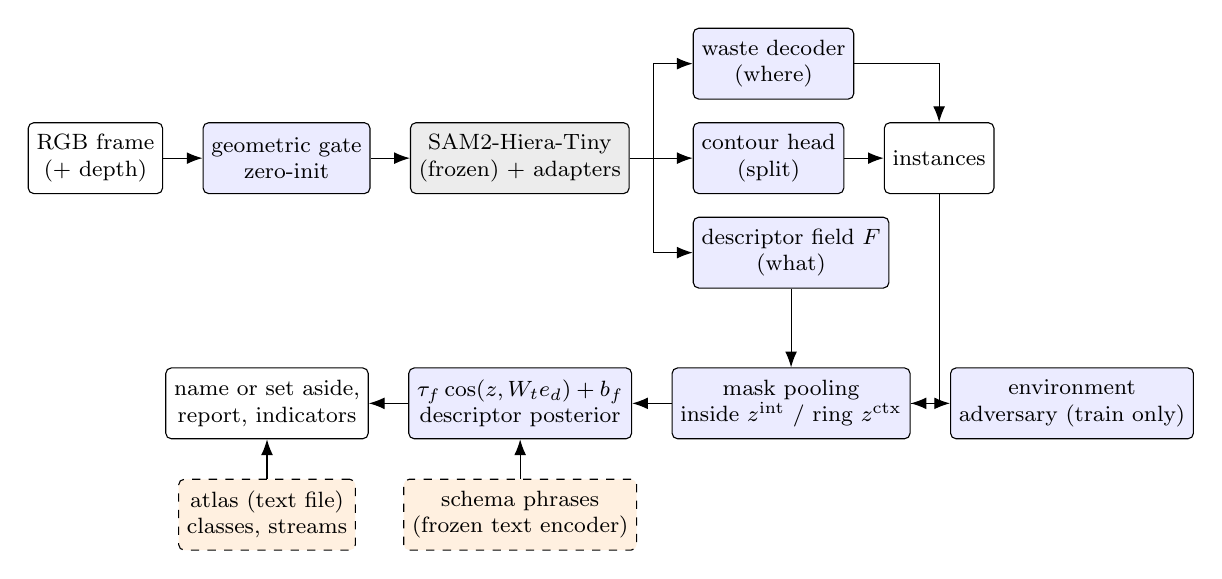
\begin{tikzpicture}[font=\footnotesize, node distance=5mm and 5mm,
  box/.style={draw, rounded corners=2pt, align=center, minimum height=9mm, inner sep=3pt},
  frozen/.style={box, fill=gray!15}, train/.style={box, fill=blue!8}, txt/.style={box, fill=orange!12, dashed},
  ar/.style={-{Latex[length=2mm]}}]
% row 1: image to heads
\node[box] (img) {RGB frame\\(+ depth)};
\node[train, right=of img] (gate) {geometric gate\\zero-init};
\node[frozen, right=of gate] (enc) {SAM2-Hiera-Tiny\\(frozen) + adapters};
\node[train, right=8mm of enc, yshift=12mm] (dec) {waste decoder\\(where)};
\node[train, right=8mm of enc] (cont) {contour head\\(split)};
\node[train, right=8mm of enc, yshift=-12mm] (desc) {descriptor field $F$\\(what)};
\node[box, right=of cont] (inst) {instances};
% row 2: pooling to name
\node[train, below=10mm of desc] (pool) {mask pooling\\inside $z^{\mathrm{int}}$ / ring $z^{\mathrm{ctx}}$};
\node[train, left=of pool] (score) {$\tau_f\cos(z,W_te_d)+b_f$\\descriptor posterior};
\node[box, left=of score] (name) {name or set aside,\\report, indicators};
\node[txt, below=5mm of score] (schema) {schema phrases\\(frozen text encoder)};
\node[txt, below=5mm of name] (atlas) {atlas (text file)\\classes, streams};
\node[train, right=of pool] (adv) {environment\\adversary (train only)};
\draw[ar] (img) -- (gate); \draw[ar] (gate) -- (enc);
\draw[ar] (enc.east) -- ++(3mm,0) |- (dec); \draw[ar] (enc) -- (cont); \draw[ar] (enc.east) -- ++(3mm,0) |- (desc);
\draw[ar] (dec) -| (inst); \draw[ar] (cont) -- (inst);
\draw[ar] (desc) -- (pool); \draw[ar] (inst) |- (pool);
\draw[ar] (pool) -- (score); \draw[ar] (schema) -- (score);
\draw[ar] (score) -- (name); \draw[ar] (atlas) -- (name); \draw[ar, dashed] (pool) -- (adv);
\end{tikzpicture}}
\caption{\trashscribe{}. Grey: frozen; blue: trained; orange, dashed: text read at inference, contributing no parameter. The adversary is used only during training. Only the scalars $\tau_f, b_f$ are specific to a descriptor \emph{field}; nothing is specific to a descriptor value or a class.}\label{fig:arch}
\end{figure}

\subsection{Canonical representation and common vocabulary}\label{sec:canonical}
Every dataset is converted by an adapter into the same sample: an RGB image, a binary waste mask (with an ignore label where needed), a list of instance masks, for each instance the name of an atlas entry or none, and, when known, the value of the contextual field \emph{surroundings} (e.g.\ ``sand, soil or pebbles'', ``a conveyor belt in a recycling plant''). Instance masks are real when the dataset provides them and connected components otherwise, in which case contours are not supervised.

The \emph{schema} is the controlled vocabulary. It has nine fields (Table~\ref{tab:schema}), each single-valued (values compete in a softmax) or multi-valued (independent yes/no), intrinsic (a property of the object) or contextual (a property of where it lies), with a weight used when naming. The current schema has 59 values. The \emph{atlas} describes each class in that vocabulary; for example, TACO's ``Clear plastic bottle'' is \{material: plastic; rigidity: semi-rigid; optics: transparent; shape: bottle-shaped; surface: glossy, printed or labelled; color: colorless; size: larger than a hand\} plus a free-text sentence and a collection stream. A field an entry does not mention is unknown for that class: it is neither supervised nor used to name it. We wrote atlases for all 60 TACO classes and the four ZeroWaste classes; datasets with a single class contribute to the waste mask and contours only. Values that appear in an atlas but not in the schema are appended to their field at inference (Sect.~\ref{sec:what}).

\begin{table}[t]
\caption{Descriptor schema. $|V|$: number of values. Contextual fields have naming weight 0.}\label{tab:schema}
\centering\footnotesize
\begin{tabular}{@{}llccp{5.0cm}@{}}
\toprule
Field & Kind & $|V|$ & Weight & Examples of values\\
\midrule
material & multi & 11 & 1.0 & plastic; paper or cardboard; metal; glass; expanded polystyrene foam\\
rigidity & single & 3 & 0.8 & rigid; semi-rigid; flexible and deformable\\
optics & single & 3 & 0.8 & transparent; translucent; opaque\\
shape & single & 11 & 1.0 & bottle-shaped; a thin film or bag; a small lid or cap; string-like\\
surface & multi & 6 & 0.5 & glossy; metallic and reflective; crumpled or wrinkled\\
color & multi & 10 & 0.3 & white; brown or beige; colorless; multicolored\\
state & single & 3 & 0.4 & intact; crushed or dented; torn or broken into pieces\\
size & single & 4 & 0.4 & tiny, smaller than a finger; hand-sized; bulky\\
surroundings & single & 8 & 0.0 & sand, soil or pebbles; pavement or road; a conveyor belt\\
\bottomrule
\end{tabular}
\end{table}

\subsection{Shared encoder and the waste decoder (where)}\label{sec:where}
The encoder is SAM2.1-Hiera-Tiny~\cite{ravi2025sam2,ryali2023hiera} with its feature pyramid, frozen. Following LENTE~\cite{anon_lente}, a bottleneck adapter $x\mapsto x + U\,\mathrm{ReLU}(Dx)$ with $U$ initialised to zero is attached after the attention of each of the 12 Hiera blocks (bottleneck 64), so the network starts exactly as the pre-trained model; low-rank updates of the attention projections~\cite{hu2022lora} are an alternative evaluated in Sect.~\ref{sec:ablation}. The patch embedding stays frozen: its filters are the part of the encoder most tied to low-level image statistics, which differ across cameras. Feature-statistics mixing~\cite{zhou2021mixstyle} is applied to the patch-embedding output during training.

The SAM2 mask decoder is trained without any prompt: it receives the not-a-point embedding and outputs one mask, the probability that each pixel is waste, at stride 4. Since every dataset annotates this mask, the decoder is shared by all of them and never sees a dataset identifier. A light contour head, fed by the stride-4 features and by the descriptor-field features, predicts object boundaries; at inference, connected components of waste pixels away from contours seed the instances and every remaining waste pixel joins its nearest seed. The cost of this step does not depend on the number of objects.

\paragraph{Geometric gate.} LENTE modulates the optical input with a gate computed from terrain elevation and slope. The waste counterpart of terrain is scene geometry: relative depth $D$ and its gradient magnitude $|\nabla D|$, from an RGB-D sensor or a monocular estimator~\cite{yang2024depthanything2}. The gate $x' = x\odot\big(1+\tanh g(D,|\nabla D|)\big)$, with the last layer of $g$ zero-initialised, is the identity at the start of training. It is optional and evaluated as an ablation.

\subsection{The descriptor field (what)}\label{sec:what}
The stride-8 and stride-16 features are fused and projected per pixel to the dimension of a frozen CLIP ViT-B/16 text space~\cite{radford2021clip}, giving a field $F\in\mathbb{R}^{512\times H/8\times W/8}$ (the visual re-projection $W_v$). Each schema value $d$ is embedded by the frozen text encoder through a small prompt ensemble (``an object made of \{\}'', ``a piece of litter made of \{\}'', \dots), giving $e_d$. For an object embedding $z$, the score of $d$ is
\begin{equation}
s(z,d) = \tau_{f(d)}\,\cos\!\big(z,\;W_t e_d\big) + b_{f(d)}, \qquad W_t e = e + A\,\sigma(B e),\label{eq:score}
\end{equation}
where $f(d)$ is the field of $d$, $A$ is initialised to zero so that $W_t$ starts as the identity on the raw text space, and $\tau_f, b_f$ are the only field-specific parameters (18 scalars in total). No parameter is indexed by a descriptor value or a class: a phrase never seen in training---a paraphrase, a new material, the value ``a face mask with ear loops'' introduced by an atlas entry---is scored through the same computation. The posterior is a softmax over the values of a single-valued field and a sigmoid for multi-valued ones.

\subsection{Intrinsic and contextual pooling}\label{sec:pool}
Given an instance mask $m_i$ resampled to the stride-8 grid as fractional coverage, the intrinsic embedding is $z_i^{\mathrm{int}} = \sum_p m_i(p)F(p)/\sum_p m_i(p)$, and the contextual embedding $z_i^{\mathrm{ctx}}$ is the average of $F$ over the ring $R_i$ obtained by dilating the support of $m_i$ by three cells (24 pixels) and removing the object itself. Intrinsic fields are scored from $z^{\mathrm{int}}$, contextual fields from $z^{\mathrm{ctx}}$. The split makes explicit, and measurable, the information that a classifier on object crops mixes implicitly: what the object is and where it lies.

\subsection{Removing the environment}\label{sec:debias}
\paragraph{Cross-dataset object transplant.} With probability $0.5$ a training sample is rebuilt by pasting up to six of its annotated objects, rescaled by a factor in $[0.6,1.3]$, onto an image from a \emph{different} dataset, with feathered alpha blending and a random partial transfer of the background colour statistics to the object. Masks of occluded background objects are updated, the surroundings label becomes that of the background image, and the object keeps its own descriptors. This breaks the object--environment correlation at the pixel level, extending copy-paste augmentation~\cite{ghiasi2021copypaste} across datasets.

\paragraph{Environment adversary.} A two-layer classifier predicts the surroundings of each object from its \emph{intrinsic} embedding through a gradient-reversal layer~\cite{ganin2015grl}, with the reversal strength ramped as $\lambda_p = 2/(1+e^{-10p})-1$ over training progress $p$. Without transplant the adversary would fight the descriptor loss whenever material and environment are correlated; with transplant the two objectives are compatible.

\paragraph{Balanced sampling.} Datasets differ by an order of magnitude in size; a dataset $k$ with $N_k$ images is drawn with probability $\propto N_k^{\alpha}$ with $\alpha = 0.5$, uniformly within it.

\subsection{Training objective}\label{sec:loss}
The loss is $\mathcal{L} = \mathcal{L}_{\mathrm{mask}} + 0.5\,\mathcal{L}_{\mathrm{contour}} + \mathcal{L}_{\mathrm{desc}} + 0.5\,\mathcal{L}_{\mathrm{dense}} + 0.1\,\mathcal{L}_{\mathrm{adv}}$. $\mathcal{L}_{\mathrm{mask}}$ is binary cross-entropy (positive weight 2) plus soft Dice on valid pixels at full resolution; $\mathcal{L}_{\mathrm{contour}}$ is weighted binary cross-entropy on datasets with real instances. $\mathcal{L}_{\mathrm{desc}}$ is, for each object and each field its class describes, a soft-target cross-entropy for single-valued fields and binary cross-entropy for multi-valued ones; a field the atlas leaves blank contributes nothing, so a missing annotation is never read as a negative. $\mathcal{L}_{\mathrm{dense}}$ applies the intrinsic part of the same loss to up to 16 stride-8 cells sampled inside each object, which makes the field usable as a per-pixel map for free-text queries. $\mathcal{L}_{\mathrm{adv}}$ is the adversary's cross-entropy.

\subsection{From a description to a name}\label{sec:naming}
Naming ranks atlas entries with three evidence streams. \emph{Descriptor agreement}, after direct attribute prediction~\cite{lampert2014dap}, compares per intrinsic field the posterior with the entry's profile by cosine, both re-weighted by an inverse document frequency over the atlas, and averages over the fields the entry describes with the field weights of Table~\ref{tab:schema}. The \emph{text prototype} of an entry is the weighted mean of the re-projected phrases $W_t e_d$ it names; it is compared with $z^{\mathrm{int}}$ directly. \emph{Prose} compares $z^{\mathrm{int}}$ with the re-projected embedding of the entry's sentence. The streams are standardised across entries for each object and averaged. Because training sharpens the classes it has seen, the fused score of every class present in training is lowered by $\gamma$ (calibrated stacking~\cite{chao2016gzsl}); $\gamma$ is the largest value that keeps 90\% of the seen-class accuracy on the \emph{validation} split, which contains no held-out class. An object is named only when the top entry clears a confidence and a margin threshold; otherwise it is \emph{set aside}. Contextual fields have weight zero throughout: the beach does not say whether an object is a bottle.

\subsection{Offline deployment and monitoring indicators}\label{sec:edge-method}
At deployment the network is exported as one graph---image in; waste probability, contour probability and descriptor field out---and compiled with TensorRT on the device. Low-rank updates, when used, are folded into the frozen weights before export. Everything else is a few matrix products on small tensors: instance extraction, pooling, scoring against a phrase matrix $W_t e_d$ precomputed on a workstation, and naming against precomputed atlas profiles and prototypes. The text encoder is therefore not needed on the device; it is needed only to embed new phrases, which happens off-line when an atlas changes. For every frame the system reports waste coverage, object count, each object's description, name or set-aside decision and collection stream, composition by material and by stream, and one sentence per object built only from scored descriptor values, so that every clause can be traced to a visual property.

%% ============================================================================
\section{Experimental setup}\label{sec:setup}

\subsection{Datasets}
Table~\ref{tab:datasets} lists the datasets. TACO and BePLi v2 have no official split; we use a fixed 70/10/20 image split (seed 42). ZeroWaste-f and MJU-Waste use their official splits; UAVVaste uses the same 70/10/20 rule. TACO scene labels are mapped to the surroundings field; the other datasets have a single surroundings value each.

\begin{table}[t]
\caption{Datasets. ``Classes'' is the native taxonomy; ``Descr.'' says whether the atlas describes its classes. \tbd{verify counts against the downloaded versions.}}\label{tab:datasets}
\centering\footnotesize
\begin{tabular}{@{}lllrcc@{}}
\toprule
Dataset & Environment & Annotation & Images & Classes & Descr.\\
\midrule
TACO~\cite{proenca2020taco} & outdoor litter, mixed scenes & instance polygons & 1{,}500 & 60 & yes\\
ZeroWaste-f~\cite{bashkirova2022zerowaste} & recycling conveyor & instance masks & \tbd{n} & 4 & yes\\
UAVVaste~\cite{kraft2021uavvaste} & aerial, low altitude & instance masks & 772 & 1 & no\\
MJU-Waste~\cite{wang2020mjuwaste} & indoor, RGB-D & instance masks & 2{,}475 & 1 & no\\
BePLi v2~\cite{bepli2023} & beach & instance masks (RLE) & 3{,}722 & 13 & \tbd{atlas}\\
\bottomrule
\end{tabular}
\end{table}

\subsection{Protocols}
\emph{E1, in-domain}: train and test on one dataset, the conventional reference. \emph{E2, multi-domain}: one model on all datasets, tested per dataset. \emph{E3, leave-one-dataset-out (LODO)}: train and select the model on four datasets, test on the fifth, which no training or selection step sees. \emph{E4, held-out classes}: seven TACO classes---Glass bottle, Pop tab, Plastic straw, Crisp packet, Paper bag, Foam cup, Egg carton---are removed from training \emph{and} validation by dropping every image that contains them (removing only their masks would teach the decoder that they are background); each is composable from descriptors that training classes carry. \emph{E5}: ablations on E4. \emph{E6}: the E4 recipe at 640\,px, the deployment resolution.

\subsection{Metrics}
Segmentation: IoU, F1, precision and recall of the waste class over valid pixels, and boundary F1 with a 2-pixel tolerance. Description: per-field mean average precision over objects whose class describes the field, against the \emph{prevalence floor}, the expected AP of a random ranking. Naming: top-1 accuracy averaged per class on seen and unseen classes, scored against all atlas entries together, and their harmonic mean $H$~\cite{xian2019gzsl}; we report the uncalibrated and the validation-calibrated operating points and the calibration-free area under the seen--unseen curve (AUSUC)~\cite{chao2016gzsl}. Retrieval: average precision of each held-out entry over the test pool, its ratio to prevalence (lift), a 2{,}000-sample bootstrap interval~\cite{efron1979bootstrap} and a 2{,}000-permutation $p$-value~\cite{ojala2010permutation}. Environment leakage: five-fold accuracy of a logistic-regression probe predicting the surroundings from $z^{\mathrm{int}}$, against the majority rate; lower is better. Edge: latency, throughput and peak memory on the device.

\subsection{Baselines}
On identical splits: SegFormer-B2~\cite{xie2021segformer} fully fine-tuned on the same data, sampler and augmentation; a training-free open-vocabulary pipeline, OWLv2~\cite{minderer2023owlv2} boxes from text queries prompting SAM2.1-Tiny; raw CLIP on object crops (1.35$\times$ the box) for description and naming; a closed-vocabulary linear probe with one weight vector per descriptor, which cannot score unseen phrases; and the LENTE recipe without descriptor head or debiasing.

\subsection{Implementation details}
Input 1024\,px (640\,px for E6), letterboxed. AdamW with learning rates $3\times10^{-4}$ (heads), $10^{-4}$ (adapters) and $5\times10^{-5}$ (decoder), weight decay $10^{-4}$, 300 warm-up steps and cosine decay; 40 epochs of 4{,}000 samples, batch 8, bfloat16 autocast; early stopping on validation IoU plus descriptor mAP (patience 8). The model has 33.78\,M parameters, of which 6.56\,M are trained: 0.61\,M adapters (2.2\% of the frozen 27.22\,M encoder), the 4.22\,M decoder, the 1.40\,M descriptor field, the 0.07\,M contour head, the 0.13\,M text re-projection and 18 field scalars; the 0.13\,M adversary is discarded after training. Training ran on \tbd{GPU}; deployment on a Jetson Orin Nano 8\,GB (JetPack \tbd{6.x}, TensorRT \tbd{10.x}, MAXN power mode). \tbd{LLM-use statement required by the journal: describe the use of AI assistance in code and text preparation here.}

%% ============================================================================
\section{Results}\label{sec:results}

\subsection{Segmentation across unseen environments}\label{sec:lodo}
Table~\ref{tab:lodo} reports waste IoU on each dataset when it is left out of training. \tbd{Text after E3: gap to in-domain, gap to SegFormer and to the zero-shot pipeline, which datasets transfer worst and why.}

\begin{table}[t]
\caption{Leave-one-dataset-out waste segmentation (IoU and boundary F1, \%). The target dataset is never used for training or model selection. In-domain (E1) is an upper reference, not a competitor.}\label{tab:lodo}
\centering\footnotesize
\begin{tabular}{@{}lccccc@{}}
\toprule
Target & OWLv2$\to$SAM2 & SegFormer-B2 & \multicolumn{2}{c}{\trashscribe{} (LODO)} & In-domain\\
 & zero-shot IoU & IoU & IoU & BF1 & IoU\\
\midrule
\tabinput{tables/tab_lodo.tex}
\bottomrule
\end{tabular}
\end{table}

\subsection{Describing objects, including unseen ones}\label{sec:describe}
Table~\ref{tab:describe} reports descriptor prediction per field on E4. \tbd{Text: open head vs closed probe vs raw CLIP vs floor; which fields are near-saturated, which near the floor and why.}

\begin{table}[t]
\caption{Descriptor prediction on E4 test objects, mean average precision per field. \emph{Floor}: prevalence; \emph{CLIP}: raw CLIP on crops; \emph{Probe}: closed-vocabulary linear head.}\label{tab:describe}
\centering\footnotesize
\begin{tabular}{@{}lcccc@{}}
\toprule
Field & Floor & CLIP & Probe & \trashscribe{}\\
\midrule
\tabinput{tables/tab_describe.tex}
\bottomrule
\end{tabular}
\end{table}

\subsection{Naming and retrieving held-out classes}\label{sec:heldout}
Table~\ref{tab:retrieval} reports retrieval of each held-out class from its atlas entry alone. \tbd{Text: lifts, permutation tests, uncalibrated vs calibrated GZSL, AUSUC, per-stream analysis, failure cases and what the schema cannot express.}

\begin{table}[t]
\caption{Retrieval of the seven held-out classes by their atlas entry, over the TACO test pool. No image of these classes reached training or validation.}\label{tab:retrieval}
\centering\footnotesize
\begin{tabular}{@{}lccccc@{}}
\toprule
Class & $n$ & AP & 95\% CI & Lift & $p$\\
\midrule
\tabinput{tables/tab_retrieval.tex}
\bottomrule
\end{tabular}
\end{table}

\subsection{Ablations and environment leakage}\label{sec:ablation}
Table~\ref{tab:ablation} isolates each component. \tbd{Text: effect of transplant and adversary on the leakage probe and on unseen naming; adapters vs LoRA; geometric gate; 640 vs 1024\,px.}

\begin{table*}[t]
\caption{Ablations on E4 (\%). Env.\ probe: accuracy of a linear probe recovering the surroundings from intrinsic object embeddings (lower is better).}\label{tab:ablation}
\centering\footnotesize
\begin{tabular}{@{}lccccccc@{}}
\toprule
Variant & IoU & Desc.\ mAP & Seen & Unseen & $H$ & AUSUC & Env.\ probe\\
\midrule
\tabinput{tables/tab_ablation.tex}
\bottomrule
\end{tabular}
\end{table*}

\subsection{Offline deployment on a Jetson Orin Nano}\label{sec:edge}
The full 640\,px graph exports to ONNX (opset 17) with a maximum absolute deviation from PyTorch below $10^{-5}$ on all three outputs. Table~\ref{tab:edge} reports on-device measurements. \tbd{Text: FP16 vs FP32 agreement (engine checked against ONNX Runtime FP32), latency split between network and post-processing, power from tegrastats, comparison with NanoSAM-style pipelines whose cost grows with the number of objects.}

\begin{table}[t]
\caption{On-device performance (Jetson Orin Nano 8\,GB, MAXN). Network-only and full-pipeline latency (pre-processing, network, instances, naming, report).}\label{tab:edge}
\centering\footnotesize
\begin{tabular}{@{}lccccc@{}}
\toprule
Backend & Size & Net (ms) & FPS & Pipeline (ms) & Mem.\ (MB)\\
\midrule
\tabinput{tables/tab_edge.tex}
\bottomrule
\end{tabular}
\end{table}

\subsection{A monitoring case}
\tbd{Qualitative figure: frames from each environment with masks, object sentences and the composition by stream; the same frames re-read with a second municipality's atlas that groups streams differently, with no retraining. Add one class written only in the atlas (e.g.\ disposable face mask) and show its retrieval.}

%% ============================================================================
\section{Discussion and limitations}\label{sec:discussion}
\tbd{Write after results. Points to address: (i) descriptor supervision is derived from class-level atlas profiles, so it is as good as the atlas and cannot capture instance-level variation (a crushed bottle is still ``intact'' in the profile when the field is set); (ii) single-class datasets train the mask but not the descriptors; (iii) transplanted objects carry the source camera's appearance, which colour harmonisation only partly removes; (iv) calibration of the seen-class bias without held-out data; (v) the leakage probe measures linear decodability only; (vi) fixed-camera video and illegal-dumping events are out of scope and complementary.}

\section{Conclusions}\label{sec:conclusions}
\tbd{Three to five sentences once the numbers are in.}

%% ============================================================================
\backmatter

\bmhead{Acknowledgements}
Omitted for double-blind review (see title page).

\section*{Declarations}

\begin{itemize}
\item \textbf{Funding:} Omitted for double-blind review (see title page).
\item \textbf{Competing interests:} The authors declare no competing interests relevant to this article.
\item \textbf{Ethics approval and consent to participate:} Not applicable. Only publicly available datasets of waste imagery were used; \tbd{state how faces and licence plates possibly present in street-level images are handled}.
\item \textbf{Consent for publication:} Not applicable.
\item \textbf{Data availability:} All datasets are publicly available from their original providers \cite{proenca2020taco,bashkirova2022zerowaste,kraft2021uavvaste,wang2020mjuwaste,bepli2023}; splits, atlases and configuration files are released with the code.
\item \textbf{Code availability:} \tbd{anonymised repository URL for review; public repository after acceptance}.
\item \textbf{Author contributions:} Omitted for double-blind review (see title page).
\end{itemize}

\bibliography{references}

\end{document}
